\documentclass[a4paper, 12pt]{extreport}

% Схемы
% Качественные характеристики (длинные строки)
% Ссылки

\RequirePackage{cmap}% Для нормальных поиска в тексте и копирования
\RequirePackage[utf8]{inputenc}
\RequirePackage[T2A]{fontenc}
\usepackage[english,russian]{babel}
\usepackage{amssymb,amsfonts,amsmath,mathtext,cite,enumerate,float}
\usepackage{pgfplots}
\usepackage{graphicx}
\usepackage{tocloft}
\usepackage{wrapfig}
\usepackage{listings}
\usepackage{caption}
\usepackage{tempora}
\usepackage{setspace}
\usepackage{geometry}
\usepackage{indentfirst}
\usepackage{pdfpages}
\usepackage{enumerate,letltxmacro}
\usepackage{threeparttable}
\usepackage{hyperref}
\usepackage{flafter}
\usepackage{enumitem}
\usepackage{multirow}

\usepackage[figure,table]{totalcount}
\usepackage{lastpage}

\setlist{nosep}

\newcommand{\ssr}[1]{\begin{center}
\LARGE\bfseries{#1}
\end{center} \addcontentsline{toc}{chapter}{#1}  }

\makeatletter
\renewcommand\LARGE{\@setfontsize\LARGE{22pt}{20}}
\renewcommand\Large{\@setfontsize\Large{20pt}{20}}
\renewcommand\large{\@setfontsize\large{16pt}{20}}
\makeatother
\RequirePackage{titlesec}
\titleformat{\chapter}[block]{\hspace{\parindent}\large\bfseries}{\thechapter}{0.5em}{\large\bfseries\raggedright}
\titleformat{name=\chapter,numberless}[block]{\hspace{\parindent}}{}{0pt}{\large\bfseries\centering}
\titleformat{\section}[block]{\hspace{\parindent}\large\bfseries}{\thesection}{0.5em}{\large\bfseries\raggedright}
\titleformat{\subsection}[block]{\hspace{\parindent}\large\bfseries}{\thesubsection}{0.5em}{\large\bfseries\raggedright}
\titleformat{\subsubsection}[block]{\hspace{\parindent}\large\bfseries}{\thesubsection}{0.5em}{\large\bfseries\raggedright}
\titlespacing{\ssr}{12.5mm}{-22pt}{10pt}
\titlespacing{\chapter}{12.5mm}{-22pt}{10pt}
\titlespacing{\section}{12.5mm}{10pt}{10pt}
\titlespacing{\subsection}{12.5mm}{10pt}{10pt}
\titlespacing{\subsubsection}{12.5mm}{10pt}{10pt}

\makeatletter
\renewcommand{\@biblabel}[1]{#1.}
\makeatother
%
%\titleformat{\chapter}[hang]{\LARGE\bfseries}{\hspace{1.25cm}\thechapter}{1ex}{\LARGE\bfseries}
%\titleformat{\section}[hang]{\Large\bfseries}{\hspace{1.25cm}\thesection}{1ex}{\Large\bfseries}
%\titleformat{name=\section,numberless}[hang]{\Large\bfseries}{\hspace{1.25cm}}{0pt}{\Large\bfseries}
%\titleformat{\subsection}[hang]{\large\bfseries}{\hspace{1.25cm}\thesubsection}{1ex}{\large\bfseries}
%\titlespacing{\chapter}{0pt}{-\baselineskip}{\baselineskip}
%\titlespacing*{\section}{0pt}{\baselineskip}{\baselineskip}
%\titlespacing*{\subsection}{0pt}{\baselineskip}{\baselineskip}

\geometry{left=10mm}
\geometry{right=10mm}
\geometry{top=10mm}
\geometry{bottom=10mm}

\onehalfspacing

\renewcommand{\theenumi}{\arabic{enumi}}
\renewcommand{\labelenumi}{\arabic{enumi}\text{)}}
\renewcommand{\theenumii}{.\arabic{enumii}}
\renewcommand{\labelenumii}{\asbuk{enumii}\text{)}}
\renewcommand{\theenumiii}{.\arabic{enumiii}}
\renewcommand{\labelenumiii}{\arabic{enumi}.\arabic{enumii}.\arabic{enumiii}.}

\renewcommand{\cftchapleader}{\cftdotfill{\cftdotsep}}

\addto\captionsrussian{\renewcommand{\figurename}{Рисунок}}
\DeclareCaptionLabelSeparator{dash}{~---~}
\captionsetup{labelsep=dash}

\captionsetup[figure]{justification=centering,labelsep=dash}
\captionsetup[table]{labelsep=dash,justification=raggedright,singlelinecheck=off}

\graphicspath{{images/}}%путь к рисункам

\newcommand{\floor}[1]{\lfloor #1 \rfloor}

\pgfplotsset{width=0.85\linewidth, height=0.5\columnwidth}

\linespread{1.3}

\parindent=1.25cm

%\LetLtxMacro\itemold\item
%\renewcommand{\item}{\itemindent0.75cm\itemold}

\renewcommand{\labelitemi}{---}
\setlist[itemize]{leftmargin=1.25cm, itemindent=0.65cm}
\setlist[enumerate]{leftmargin=1.25cm, itemindent=0.55cm}

\newcommand{\specialcell}[2][c]{%
    \begin{tabular}[#1]{@{}c@{}}#2\end{tabular}}

\frenchspacing

\begin{document}
    \pagestyle{empty}

    \ssr{Методы оптимизации первого порядка}

    \textbf{Задача оптимизации.} Для задачи оптимизации, удобной для решения методами
    математического программирования, необходимо минимизировать (или максимизировать)
    вещественнозначную функцию $f(x)$, зависящую от $n$-мерного аргумента $x$.
    Компоненты $x$ должны удовлетворять системе ограничений, состоящей из
    уравнений $H_k(x) = 0$, где $k = 1, 2, ..., m$, или неравенств $g_j(x) \geq 0$,
    где $j = m + 1, ..., s$. Математически это можно записать следующим образом: $\min_{Q} f(x)$
    или $\max_{Q} f(x)$, где область допустимых решений $Q$
    определяется как: $H_k(x) = 0, k = 1, 2, ..., m$ и $g_j(x) \geq 0, j = m + 1, ..., s$[1].

    В математической формулировке задачи условной оптимизации целевую функцию выбирают
    с таким знаком, чтобы решение задачи соответствовало поиску минимума.
    Поэтому стандартная запись задачи математического программирования выглядит следующим
    образом: $\min_{Q} f(\vec{x})$[1].

    \textbf{Методы решения первого порядка.}
    Методы 1-го порядка используют информацию о производной функции.
    Если ограниченная снизу целевая функция $f(x)$, $x$ $\in$ $R^n$ является
    дифференцируемой на множестве $R^n$, то алгоритм поиска точки $x^*$ ее минимума
    можно построить, используя информацию, по крайней мере, о градиенте этой функции[1].
    К таким методам относятся метод наискорейшего спуска, касательных, Больцано, методы сопряженных градиентов и др.

    \textbf{Метод наискорейшего спуска}. Метод заключается в выборе направления поиска,
    совпадающего с антиградиентом функции $-\nabla f(x)$, так как это направление
    обеспечивает наиболее быстрое убывание. На каждом шаге решение обновляется по
    формуле \ref{eq:a}, где $\lambda_k$ — оптимальный шаг,
    минимизирующий функцию вдоль данного направления. Итерации продолжаются до тех пор,
    пока изменение $\|x_{k+1} - x_k\|$ не станет меньше заданного порога $\varepsilon$[3].

    \vspace{-10pt}
    
    \begin{equation}
        \label{eq:a}
        x_{k+1} = x_k - \lambda_k \nabla f(x_k)
    \end{equation}

    \textbf{Метод касательных}.
    Пусть функция $f(x)$ выпукла и дифференцируема на отрезке $[a, b]$.
    Если $f'(a) > 0$ или $f'(b) \leq 0$, то $a$ либо $b$ является точкой
    минимума соответственно, и тогда задача решена, поэтому примем $f'(a) < 0$, $f'(b) > 0$.
    Примем $a_1 = a$, $b_1 = b$.
    Далее строим касательные к графику $f(x)$ в точках $a_1$ и $b_1$ и находим точку
    их пересечения, обозначим её $c_1$.
    Если $f'(c_1) > 0$, то принимаем $a_2 = a_1$, $b_2 = c_1$.
    Если $f'(c_1) < 0$, то принимаем $a_2 = c_1$, $b_2 = b_1$.
    Если $f'(c_1) = 0$, то задача решена и точка $c_1$ является искомой.
    Повторяем процедуру до тех пор, пока не выполнится критерий остановки.
    На рис. \ref{fig:figure} показано три итерации метода касательных[2].
    \begin{figure}[h]
        \centering
        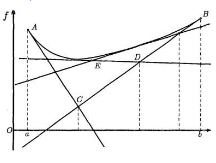
\includegraphics[scale=0.5]{img}
        \caption{Геометрическая иллюстрация метода касательных.}
        \label{fig:figure}
    \end{figure}

    \textbf{Список использованных источников}

    \begin{enumerate}
        \item Методы безусловной оптимизации : Тексты лекций. / Т. М. Попова; [науч. ред. Р. В. Намм]. - Хабаровск: Изд-во Тихоокеан. гос. ун-та, 2013. – 76 с.
        \item Методы оптимизации: Учеб. пособие / Аббасов М. Э. - СПб.: Издательство “ВВМ”, 2014. - 64 с.
        \item Методы многомерной безусловной минимизации : учеб. посо-
        бие по курсу «Методы оптимизации» / В. П. Северин. – Х. : НТУ
        «ХПИ», 2013. – 160 с.
    \end{enumerate}
\end{document}